\clearpage
\cxset{header style=empty}
\chapter{SAMPLE HEADERS AND FOOTERS}

%\section{Using the fancyvrb package}
%
%Most LaTeX users, when redesigning running headers or footers will use the fancyvrb package. This well established package by Piet van
%Oostrum, allows easy customization of page headers and footers. The default page style provided by fancyhdr is named fancy. It should be activated via
%\lstinline{\pagestyle} after any changes to textwidth are made, as fancyhdr initializes
%the header and footer widths using the current value of this length.
%The look and feel of the fancy page style is determined by six declarations
%Balle 1I1[l'rtace that define the material that will appear on the left, center, and right of the header
%and footer areas. For example, lhead specifies what should show up on the left
%in the header area, while cfoot defines what will appear in the center of the
%footer area. The results of all six declarations are shown in the next example.
%
%\section{Header and footer options of the chaptersx package}
%
%To keep a consistent and familiar interface, the package uses the
%fancyhdr package which it loads by default and defines option keys that are similar to the macros provided by fancyhdr, as well as some additional typesetting keys.
%
%It is also possible to group these in styles, which we have done for the following:
%
%We have endeavoured o include as many keys possible in order to provide a consistent and comprehensive style.
%
%\section{Example header style}


\section{Description of the header engine}

The header engine works by defining three vertical regions to contain a top and bottom rule or other material and a middle layer that contains the text and or graphical material. In its simpler form is an assembly of boxes as shown in figure~\ref{fig:headerengine} .
\medskip

\noindent\vbox{

\framebox[80pt]{toprule}

\fbox{\fbox{offset}$\rightarrow$\fbox{\fbox{name} \fbox{number} \fbox{title} \fbox{page number}}}

\framebox[80pt]{bottomrule}

\captionof{figure}{Typical assembly of boxes for a header}
\label{fig:headerengine}
}

Of course the order of display of the various components can vary, for example in figure~\ref{fig:headerengine01}, we have the page number to the left.

\noindent\fbox{\vbox{%
oddhead\par
\framebox[80pt]{toprule}

\fbox{\fbox{offset}$\rightarrow$\fbox{\fbox{page number}\fbox{name} \fbox{number} \fbox{title} }}

\framebox[80pt]{bottomrule}

\captionof{figure}{Typical assembly of boxes for a header}
\label{fig:headerengine01}
}}

The LaTeX engine as previously described allows for an oddhead and evenhead macros to hold the typesetting information. The typesetting information is obtained asynchrnously,

The chaptermark assembles and stores

\fbox{\fbox{chapter name}$\rightarrow$\fbox{chapter number}$\rightarrow$\fbox{chapter title}}

whereas the sectionamark similarly stores information on section numbering:

\begin{figure}[h]
\fbox{\fbox{section name}\fbox{section number}\fbox{section title}}
\end{figure}

This information of the mark macros is then activated by the leftmark and rightmark commands and when the typesetter calls the oddhead and evenhead the page number is added. So to have a complete definition
we need to define both the marks as well as the oddhead and evenhead macros. Similarly the pagenumber's position can vary in different designs.

The approach we took is to firstly extend the informtion held in each box, for example, the chaptername
looks more like:

\begin{figure}[h]
   \fbox{chaptername before}$\rightarrow$\fbox{chaptername}$\rightarrow$\fbox{chapternameafter}
\end{figure}

Similarly the header elements, \textit{name, number, title} and \textit{pagenumer}  hold information to add material before and after the element. This adds complexity, but generalizes and abstracts the problem nicely.

Now back to leftmarks and rightmarks. The leftmark or rightmark is called by the oddside or evenside macros. We suitably add macros for before and after.

\fbox{before mark}$\rightarrow$\fbox{leftmark or rightmark}$\rightarrow$\fbox{after mark}

\subsection{Discussion}

One would argue that this is a convoluted way of describing the header and footers. However, to have a truly flexible system (with no macro writing for designers and authors) one has to resort to such a long way. It is in many respects simlar to CSS. A looks description language needs as many variables and as much flexibility as possible. The one up on CSS is that the template can be saved and themes developed and invoked very simply.

\subsection{Example settings}
\index{Styles!style56}
\index{Header and footers!example}
To define a style based on the \textit{headings} pagestyle. We will base the style definition on figure~\ref{globalstrategy}. The interesting part of this design is that the chapter numbers are not shown shown in the introduction (which is treated as front matter material). The rest of the chapters are numbered, although the header information and styling remains the same.

\begin{figure}[hp]
\centering
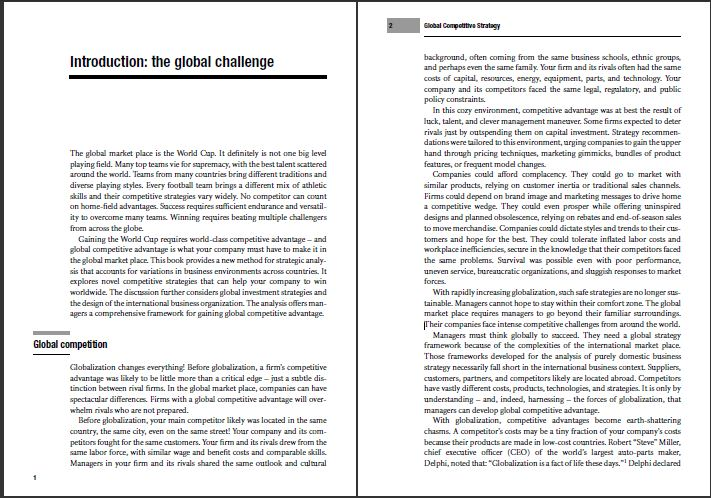
\includegraphics[width=0.8\textwidth]{chapter56}\vspace{0.5\baselineskip}
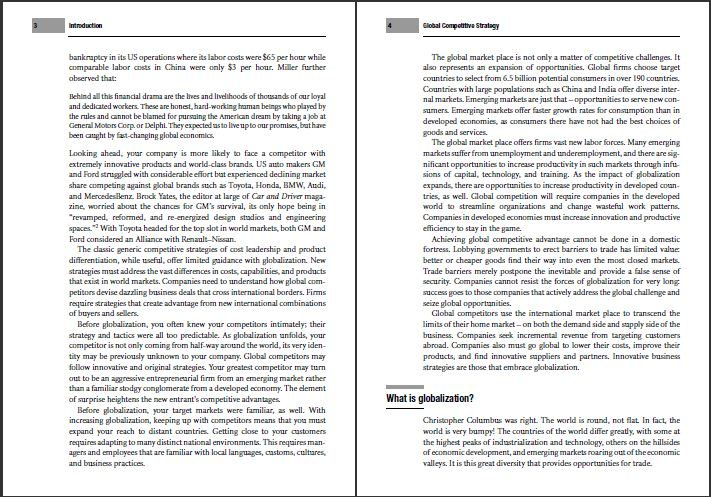
\includegraphics[width=0.8\textwidth]{chapter56a}
\caption{Example pages from \textit{Global Competitive Strategy}, by Daniel F. Spulber,} Cambridge University Press, 2007.
\label{globalstrategy}
\end{figure}

The interesting part of this design is that the headers as well as the chapter openings vary. On the even page the words ``Golbal Competitive Strategy'' are printed, which is the book title\footnote{Although it is an attractive design, it does not mean that this way of header information is a good way of structuring information.}.

Note that since LaTeX only provides two mark we need to arrange our own typesetting rules, we will abuse the macros to achieve it.

\begin{tcolorbox}
\begin{lstlisting}
\cxset{headings style56/.style={
          pagestyle=headings,
          header style=headings,
% Chaptermarks
          chaptermark name color=black,
          chaptermark after number=,
          chaptermark name=SHORT BOOK TITLE,
          chaptermark numbering=none,
          chaptermark title color=black!80,
          chaptermark title before=\@gobble,
% Leftmarks
          leftmark before=\colorbox{thegray!50}{\thepage\quad}\quad, %even pages
          leftmark after=\hfill\hfill,
% Right marks influenced by chapter name?
          rightmark before=\colorbox{thegray!50}{\thepage\quad}\quad, %odd pages
          rightmark after=\hfill\hfill,
% Section marks
          sectionmark name custom=\chaptertitle@cx,
          sectionmark number=none,
          sectionmark name color=black,
          sectionmark title color=black!80,
          sectionmark before title=\@gobble, % we do not need the section title
          sectionmark after title=\hfill\hfill,
          sectionmark after number=,
%  rules we remove or inherit
%       header top rule=false,
          header bottom rule=true,
          header offset even=-1.3cm,
          header offset odd=-1.3cm,
          }}
\end{lstlisting}
\end{tcolorbox}

The approach we need to take here is to first define the even pages, which contain the book short title. Instead of printing the \cs{chaptername}, we give the value of the title to the \textbf{chaptermark} key.

\begin{tcolorbox}
   chaptermark name = SHORT BOOK TITLE,
\end{tcolorbox}

Offsetting the page numbers is done by using the \textbf{header offset} key. As both the left as well as the right pages have the page on the left we offset both of them by the same amount.

\begin{tcolorbox}
\begin{lstlisting}
    chaptermark name = SHORT BOOK TITLE,
    header offset even = -1.3cm,
    header offset odd  = -1.3cm,
\end{lstlisting}
\end{tcolorbox}

\subsection{Inheriting and transforming styles}
One of the advantages of this method, is that we can inherit styles and transform styles easily. Consider style57, which is shown in figure. This is a simple design and follows trends to include the book title in the header. This is a very similar design to header \textit{style57}.

\begin{tcolorbox}
\begin{lstlisting}
%% STYLE 57 QUANTUM FRONTIER
\cxset{headings style57/.style={
          headings style56,
% Chaptermarks
          chaptermark name={\bfseries The Quantum Frontier},
% Leftmarks
          leftmark before=\thepage\quad, %even pages
          leftmark after=\hfill\hfill,
% Right marks influenced by chapter name?
          rightmark before=\hfill\hfill, %odd pages
          rightmark after=\thepage,
% Section marks
          sectionmark name custom=\chaptertitle@cx,
          sectionmark after title=\quad,
%  rules we remove or inherit
          header top rule=false,
          header bottom rule=false,
          header offset even=0pt,
          header offset odd=0pt,
          }}
\end{lstlisting}
\end{tcolorbox}

A crude form of object inheritance is possible by including a style at the top of the key definitions in this case \texttt{headings style56}, we then only need to redefine the values for the changes. We also set zero all offsets and adjust the widths.

The success of the method is defining an appropriate set of general commands and building a community chest of styles.

This concludes the long excursion into headers and footers. This class and method of styling is brand new and is bound to evolve, as it is being used. Feedback is most welcomed as well as bug reports.
\begin{figure}[tp]
\centering
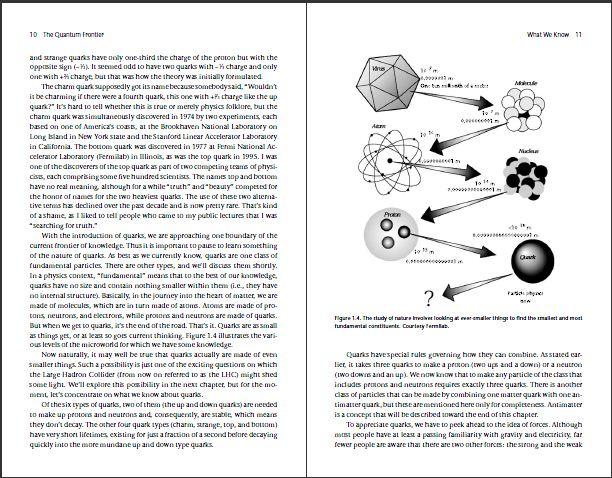
\includegraphics[width=0.8\textwidth]{chapter57a}\vspace{0.5\baselineskip}
\caption{Example pages from \textit{The quantum frontier: the large hadron collider}, by Don Lincoln, The Johns Hopkins University Press, 2009.  It uses the book short-title at even pages and the chapter title at the odd pages.}
\end{figure}

\section{Another inheritance example}

This example is from the book \textit{Evolution of the Insects} by David Grimaldi and Michael S. Engel and published by the Cambridge University Press in 2005. It is a beautifully typeset book and a fine piece of scientific work. The only difference in the headers of the previous examples is the setting of the page number and header text. This one as well as many other books uses the title of the book and the chapter name.

\begin{tcolorbox}
\begin{lstlisting}
%% EVOLUTION OF THE INSECTS
\cxset{headings style58/.style={
          headings style57,
          chaptermark name={\bfseries EVOLUTION OF THE INSECTS},
          leftmark before=\thepage\quad\hfill\hfill, %even pages
          leftmark after=,
          rightmark before=, %odd pages
          rightmark after=\hfill\hfill\thepage,
 }}
\end{lstlisting}
\end{tcolorbox}

Since most of the information was captured in \textit{style57} we inherit the values and only supply the ones  that are changing. This involves changing six settings, illustrating the strength of the procedure adopted. Just a word of caution I found it difficult to follow some of the terminology, if you confused by what a leftmark and right mark are think of them as holding all the header information except the page number.



\begin{figure}
\centering
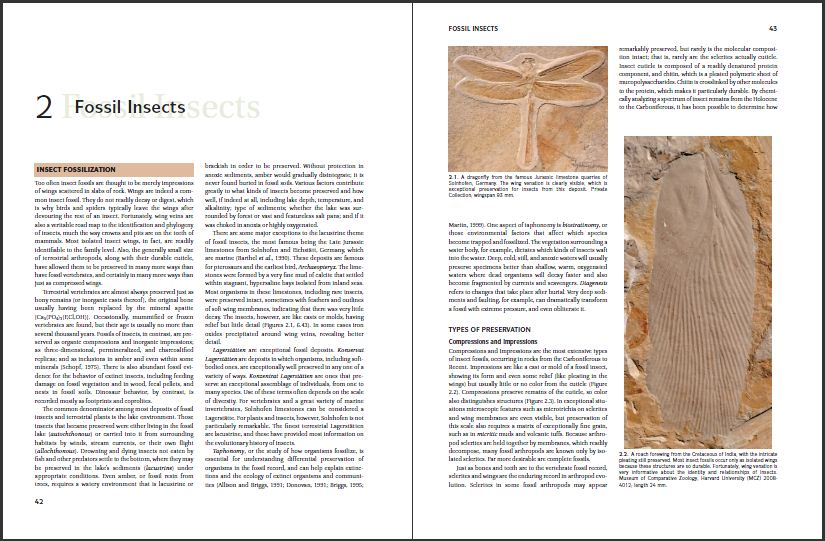
\includegraphics[width=0.8\textwidth]{chapter58}\vspace{0.5\baselineskip}
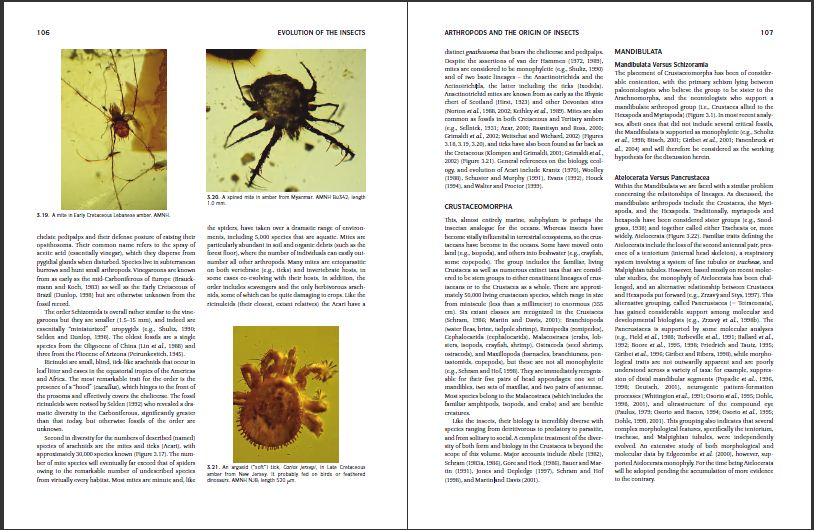
\includegraphics[width=0.8\textwidth]{chapter58a}
\caption{This example is from the book \textit{Evolution of the Insects}, David Grimaldi and Michael S. Engel,  Cambridge University Press, 2005. It is a beautifully typeset book and a fine piece of scientific work. The only difference in the headers of the previous examples is the setting of the page number and header text. This one as well as many other books use the title of the book and the chapter name in headers. The footers are empty with th exception of the chapter page}
\end{figure}


\begin{figure}
\centering
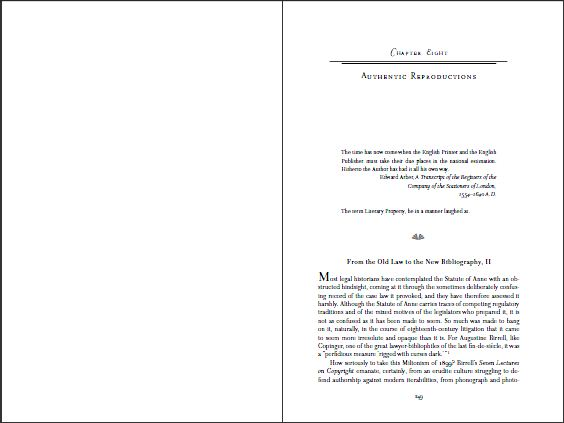
\includegraphics[width=0.8\textwidth]{chapter55}\vspace{0.5\baselineskip}
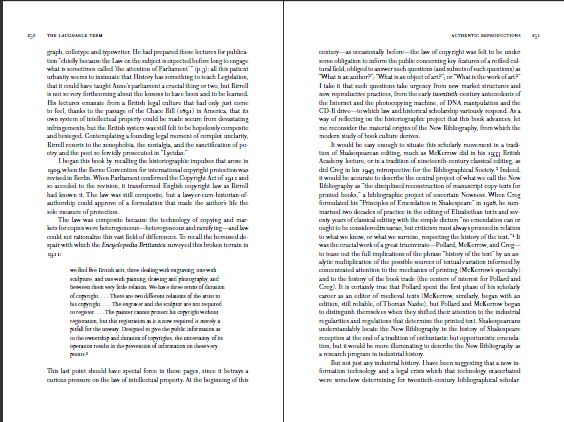
\includegraphics[width=0.8\textwidth]{chapter55a}
\caption{Example pages from \textit{The Author's Due, Printing and the Prehistory of Copyright}, by Joseph Lowewenstein, The University of Chicago Press, 2002.  It uses the part title on the even page and the chapter title on the odd page. The page number is set in the margin. The footers are clear.}
\end{figure}


\clearpage
\thispagestyle{empty}


%%%%%%%%%% NEW GEOMETRY
\newgeometry{top=1cm,bottom=2cm,left=2cm}

%% GENETICS
\makeatletter
\@specialfalse
\makeatother
\cxset{
 custom=,
 name={CHAPTER CONCEPT},
 numbering=none,
 number font-size=,
 number font-family=,
 number font-weight=,
 number color=white,
 numbering=arabic,
 chapter opening=right,
 chapter color={black},
 chapter font-family=\sffamily,
 chapter font-size=\large,
 chapter font-weight=\bfseries,
 title font-family=\sffamily,
 title font-color=teal,
 rule off,
}

\begin{specialchapter}[
     image=genetics-dogs,
     image caption={Labrador retriever\\
         puppies expressing\\
         brown (chocolate),\\
         golden (yellow),\\
         and black\\
         coat colors,\\
         traits controlled\\
         by two gene pairs.}]%
{Extensions\\ of Mendelian\\ Genetics}
\begin{itemize}
\item While alleles are transmitted from parent to   offspring
according to Mendelian principles, they often do not
display the clear-cut dominant/recessive relationship
observed by Mendel.
\item In many cases, in a departure from Mendelian genetics,
two or more genes are known to influence the phenotype
of a single characteristic.
\item Still another exception to Mendelian inheritance occurs
when genes are located on the X chromosome, because one
of the sexes receives only one copy of that chromosome,
eliminating the possibility of heterozygosity.
\item Phenotypes are often the combined result of genetics and
the environment within which genes are expressed.
\item The result of the various exceptions to Mendelian principles
is the occurrence of phenotypic ratios that differ from those
produced by standard monohybrid, dihybrid, and trihybrid
crosses.
  \end{itemize}
\end{specialchapter}


%%%%%%%%%% NEW GEOMETRY
\newgeometry{top=2cm,bottom=2cm,left=2cm}
\clearpage

\begin{tcolorbox}
\begin{lstlisting}
%% Special Chapter command
\newcommand\specialchapter@cx[2][]{%
\refstepcounter{chapter}
\cxset{image/.store in=\image@cx,
       image caption/.store in=\caption@cx}
\cxset{#1}
\vbox to 0pt{\color{blue}\rule{\paperwidth}{0.4pt}\par\vskip-1.4pt
\rule{0.4pt}{\textheight}\rule{4cm}{0.4pt}}

\vbox to 0pt{\parbox[b]{4.7cm}{%
\raggedright

\leftskip1.5cm
\caption@cx\par
 \expandafter\rule{\rulewidth@cx}{5.8cm}
}\parbox[b]{0.5cm}{
\includegraphics[width=0.5cm,height=9.15cm]{./chapters/shadow}}\includegraphics{./chapters/\image@cx}\par}

\vspace{8.2cm}
\hspace*{-3.51cm}\hbox to 0pt{\hspace*{1.01cm}
\includegraphics[width=7.7cm,height=3.8cm]{./chapters/genetics-band}
\hspace*{-2.7cm}\sffamily\color{\numbercolor@cx}\HHUGE \raise30pt\hbox{\thechapter}%
\hspace{1.5cm}\raise0.5pt\hbox{
\includegraphics{./chapters/chapterconcept}
\includegraphics{./chapters/shadow2}}
}

%% Title name
\parbox[b]{0.45\textwidth}{%
  \titlefontsize@cx
  \titlefontweight@cx
  \titlefontfamily@cx
  \leftskip0.5em \color{\titlefontcolor@cx}
  #2
}
%% Concepts
}

\newenvironment{specialchapter}[2][]{%
  \if@openright\cleardoublepage\else\clearpage\fi
    \thispagestyle{plain}%
    \global\@topnum\z@
    \@afterindentfalse
    \specialchapter@cx[#1]{#2}
    \begin{minipage}{0.5\textwidth}%
    \vspace{0.5\baselineskip}
    \raggedright
}{\end{minipage}}
\end{lstlisting}
\end{tcolorbox}


The aim of the package is to allow easy styling of chapter heads and extends these to include images and special effects, which are difficult to achieve using traditional methods.

Abstracting the various designs is a non-trivial undertaking due to the hundreds of different possibilities.

\begin{multicols}{2}
\long\def\specialsection#1{\hspace*{0.5em}\vbox{\hsize\columnwidth%
 \vspace{\baselineskip}
\refstepcounter{section}
\parindent0pt
\raggedright
\vbox to 0pt{%
\parindent0pt
\color{red}\rule[-49.6pt]{0.4pt}{50pt}%
\color{red}\rule{0.5in}{0.4pt}\colorbox{teal}{\color{white}{\large \space\thesection\space}}}%
\vskip5pt%
\hspace{-3.5pt}\fbox{.}\par
\vspace*{-45pt}
\hspace*{1em}\vbox{\Large\sffamily#1\par}}
\vspace*{\baselineskip}\par
}

\specialsection{The Ratio of Males to Females\\ in Humans is not 1.0}
\lipsum[2-5]
\specialsection{Variation in Chromosome Number:\\
Terminology and Origin}
\lipsum[1]
\bigskip
\noindent\textcolor{teal}{\large\bfseries\sffamily Monosomy}
\smallskip

\noindent\lipsum[2-3]


\specialsection{Background to the\\
sectioning commands}

The \LaTeX2e\ method of constructing the layout for Chapters is complicated and spread all over the book.cls code. Although not very difficult to customize, customization is not user friendly.

\begin{description}
\item [counters] Counters can be displayed or not. These are constructed using the normal LaTeX method.
   \begin{verbatim}
   \renewcommand \thechapter {\@arabic\c@chapter}
   \end{verbatim}

\item [name] Here we use the term \textit{name} to denote in english the word ``chapter''. This can be typeset differently, depending on the language. It depends on on redefining one macro.
   \begin{verbatim}
     \def\chaptername{Chapter}
   \end{verbatim}
\item [openright] The global option open right, triggers the typesetting of chapter on odd pages only. There are a  couple of layouts that must be typeset on an even pages.

\item [\string\chapter] The chapter command is the main author command and where all the branching starts.
    \begin{verbatim}
\newcommand\chapter{%
  \if@openright\cleardoublepage\else\clearpage\fi
    \thispagestyle{plain}%
    \global\@topnum\z@
    \@afterindentfalse
    \secdef\@chapter\@schapter}
    \end{verbatim}

One limitation for this command is that it always starts a chapter on a new page and the macro needs to be rewritten if for example a new chapter is allowed to start anywhere.

Consider options openright, openleft, continuous.

The pagestyle is also settled here.

secdef will define basic macros for chaapter and starred chapter. What it basically does... this will become unecessary as we are going to find out a bit later on, but first the @chapter.

\item [\string\@chapter] This is the basic routine
\begin{verbatim}
\def\@chapter[#1]#2{
  \ifnum \c@secnumdepth >\m@ne
    \if@mainmatter
      \refstepcounter{chapter}%
      \typeout{\@chapapp\space\thechapter.}%
      \addcontentsline{toc}{chapter}%
         {\protect\numberline{\thechapter}#1}%
      \else
         \addcontentsline{toc}{chapter}{#1}%
    \fi
  \else
    \addcontentsline{toc}{chapter}{#1}%
  \fi
  \chaptermark{#1}%
  \addtocontents{lof}{\protect\addvspace{10\p@}}%
  \addtocontents{lot}{\protect\addvspace{10\p@}}%
  \if@twocolumn
    \@topnewpage[\@makechapterhead{#2}]%
  \else
    \@makechapterhead{#2}%
    \@afterheading
  \fi}
\end{verbatim}
  The important branching command here is makechapterhead,   which is responsible for typesetting the layout.

\end{description}
\end{multicols}


\section{Counters}
\begin{verbatim}
\renewcommand \thepart {\@Roman\c@part}
\renewcommand \thechapter {\@arabic\c@chapter}
\end{verbatim}



\section{major components}

The major components of a chapter opening, is the chapter name, the number and the title. It can be enclosed in boxes rules or other decorative elements.

One peculiarity is how to specify the position of the number.

leftofchaptername rightofchaptername ownline

\subsection{algorithmic approach}

The strategy in abstracting the chapter commands follows closely to that of laTeX.

First the chapter is called with the minimum of redefinitions. This then calls makechapterhead.


\begin{specialchapter}[
     image=genetics-dogs,
     image caption={Labrador retriever\\
         puppies expressing\\
         brown (chocolate),\\
         golden (yellow),\\
         and black\\
         coat colors,\\
         traits controlled\\
         by two gene pairs.}]%
{Sample\\ Chapter\\ Styles}
\begin{itemize}
\item The many permutations of variables affecting a chapter design, necessitate an interface that is easy to use and remember. The package provides an interface that a design can simply be changed by changing one word.
\item Learn how to select from a number of predefined styles, which you can view in the pages that follow.
\item Learn how to design your own styles and incorporate them easily in a new document.
\item The designs that follow have been selected from actual books. They may differ slightly in page geometry, spacing and fonts as I have tried to keep a somewhat unified design across this document.
\item i welcome contributions in terms of libraries and additional styles. What I have provided in this package is only a very small subset of what is possible to achieve.
\item Almost all styles are numbered, as this was the easiest way to incorporate so many designs. The few exceptions are noted in the relevant pages.
  \end{itemize}
\clearpage
\end{specialchapter}
